	% Darmstadt|Frankfurt|JuanLesPins
	
	\documentclass{beamer}
	\setbeamertemplate{navigation symbols}{}
	
	\usetheme{hpi}
	\usepackage[ngerman]{babel}
	\usepackage[utf8]{inputenc}
	\usepackage{geometry}
	\usepackage[T1]{fontenc}
	\usepackage{graphicx} %Zum Bilder einbinden
	\usepackage{float} %Damit die Figures, also die Bilder, mitten im Text, an geforceter Position erscheinen
	\usepackage{verbatim} %für mehrzeilige Kommentare \begin~\end{comment}
	\usepackage{amstext} % \text{asdf} in Formeln, statt \mbox, weil mbox die Schriftgröße festsetzt	
	\usepackage{amsmath}
	\usepackage{amssymb}
	\usepackage{ucs}
	\usepackage{BeamerColor}
	
	\usepackage{listings}
	\usepackage{color}
	\usepackage{hyperref}
	\usepackage{acronym}
	\definecolor{tplcolor}{HTML}{F6AE15}
	\usecolortheme[named=tplcolor]{structure}
	
	\lstset{
		language=Java, 
		inputencoding=utf8,
		tabsize=2,
		basicstyle=\tiny,
		captionpos=b,language=JAVA,breaklines=true,      % the size of the fonts that are used for the line-numbers,
		stepnumber=5,   
		keywordstyle=\color{brown},
		commentstyle=\color{DarkGreen}, 
		stringstyle=\color{blue},
		showstringspaces=false,
		breaklines=true
		literate=%
		{Ö}{{\"O}}1
		{Ä}{{\"A}}1
		{Ü}{{\"U}}1
		{ß}{{\ss}}1
		{ü}{{\"u}}1
		{ä}{{\"a}}1
		{ö}{{\"o}}1
		{~}{{\textasciitilde}}1	
	}

	\beamersetuncovermixins{\opaqueness<1>{25}}{\opaqueness<2->{15}}
	
	\usecaptiontemplate{
	\tiny
	\structure{\insertcaptionname~\insertcaptionnumber:}
	\insertcaption
	}
	
	\usefootnotetemplate{
	\tiny
	\parindent 1em\noindent
	\hbox to 1.8em{\hfil\insertfootnotemark}\insertfootnotetext
	}
	\begin{document}
			
	\setbeamercovered{invisible}
	
	\title[Review - Entwurfsprojekt]{Review - Entwurfsprojekt\\ Eine Logistiksoftware für MöbelCorp}
	\author{Gruppe 3}
	
	 \begin{frame}[title=Hauptgebaeude_Nacht.jpg]
	 	\maketitle
	 	\date{26. Mai 2018}
 	\end{frame}
	 
	\begin{frame}
		\frametitle{Gliederung}
		\tableofcontents
		%Folien mit einem * im Titel sollen beim Vortrag übersprungen werden.
	\end{frame}
	\section*{Annahmen}
	\begin{frame}{Annahmen}
	Es wurden folgende Annahmen für das erstellte Modell getroffen:
	\begin{itemize}
		\item Der Datentyp \textbf{typ\_und\_menge} kann als Materialeintrag bezeichnet werden.
		\item Mit Material ist Materialvorrat gemeint.
		\item Der Zeitrahmen eines Projektes entspricht der Lieferfrist.
		\item Ist das Zeitlimit bei einer Anfrage 0, dann gibt es kein Zeitlimit.
		\item Artikelbezeichnungen können Buchstaben enthalten.
		\item Großhändlernamen können nicht geändert werden.
		\item \textbf{date} ist ein primitiver Datentyp.
	\end{itemize}
	\end{frame}
	\section{Abstrakte Architektur}
	\begin{frame}{Abstrakte Architektur}
		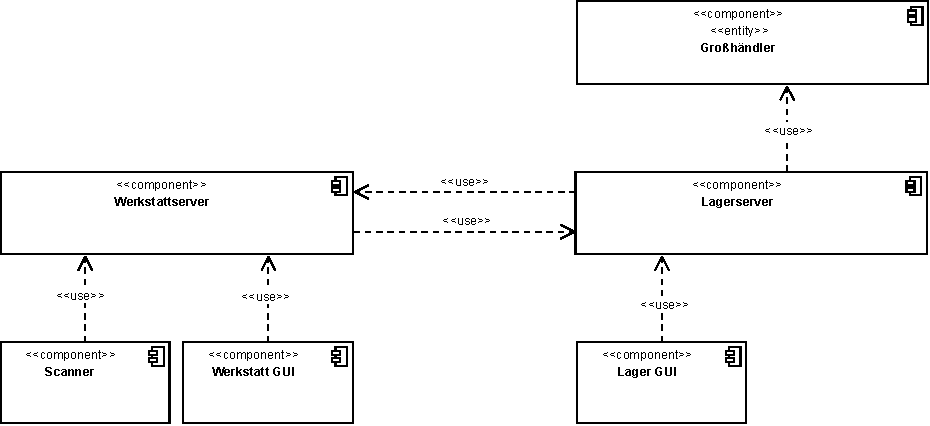
\includegraphics[width=\textwidth]{PDF/abstrakte_Architektur.pdf}
	\end{frame}
	\section{Interaktion der Komponenten}
	\begin{frame}{Use Case 1 - Bestand dokumentieren}
	Ein Werkstattmitarbeiter scannt einen Barcode. Nachdem das Material des gescannten Barcodes angezeigt wurde, wird das Material gezählt und ein Bestand eingegeben und bestätigt. Draufhin wird der \textbf{Bestand übermittelt} (vom Scanner an den Server):\\
\medskip
\texttt{sendeBestand(kennung : string, menge : int)}
\\
\medskip
Intern rechnet der Werkstattserver nun den Bedarf aus und fügt ihn der Anforderungsliste hinzu.
\end{frame}
	\begin{frame}{Use Case 2 - Auftrag eintragen}
		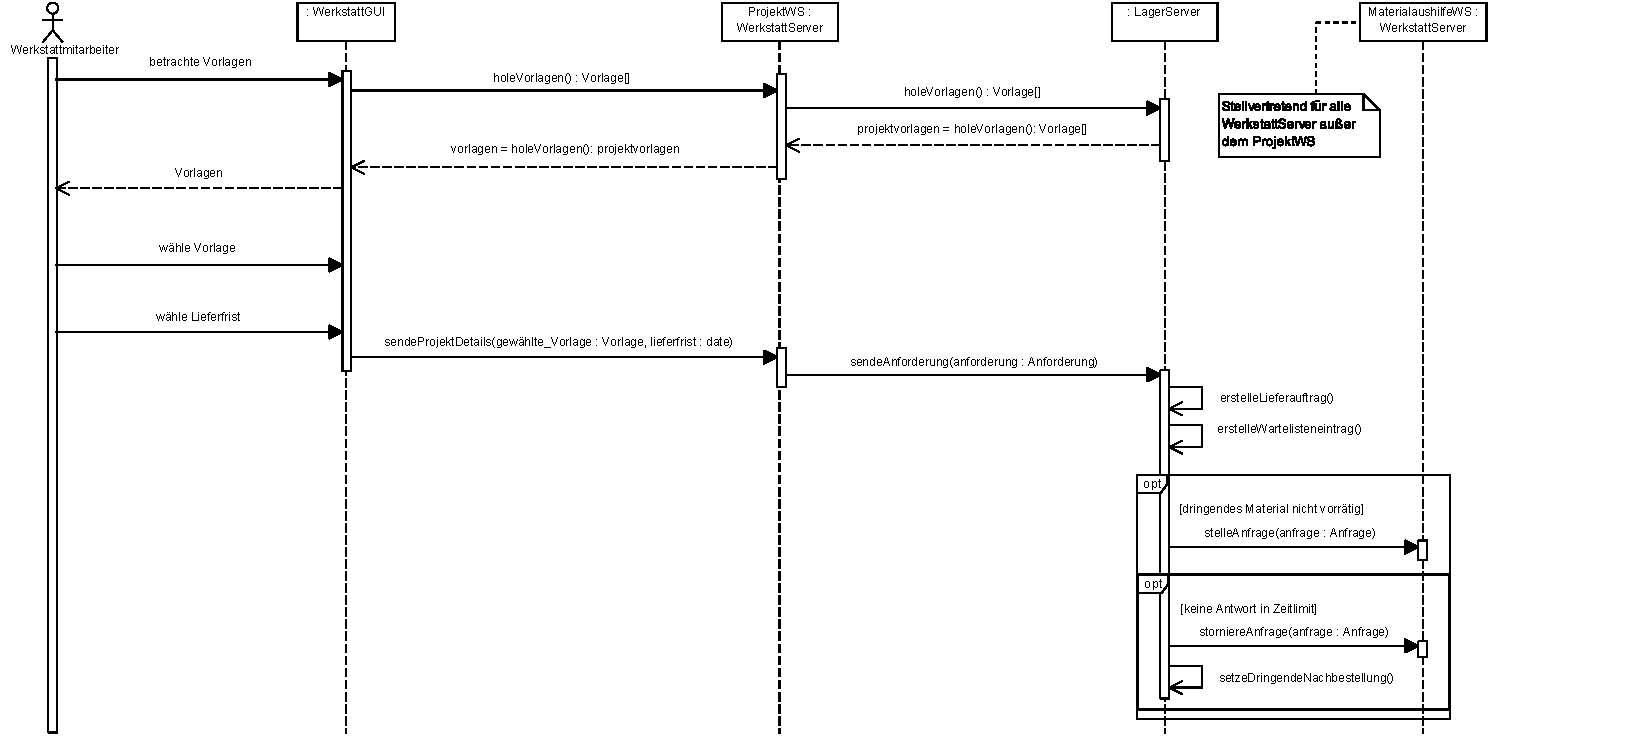
\includegraphics[width=\textwidth]{PDF/Use_Case_2-Auftrag_eintragen.pdf}
	\end{frame}
	\begin{frame}{Use Case 3 - Materialanfrage beantworten}
		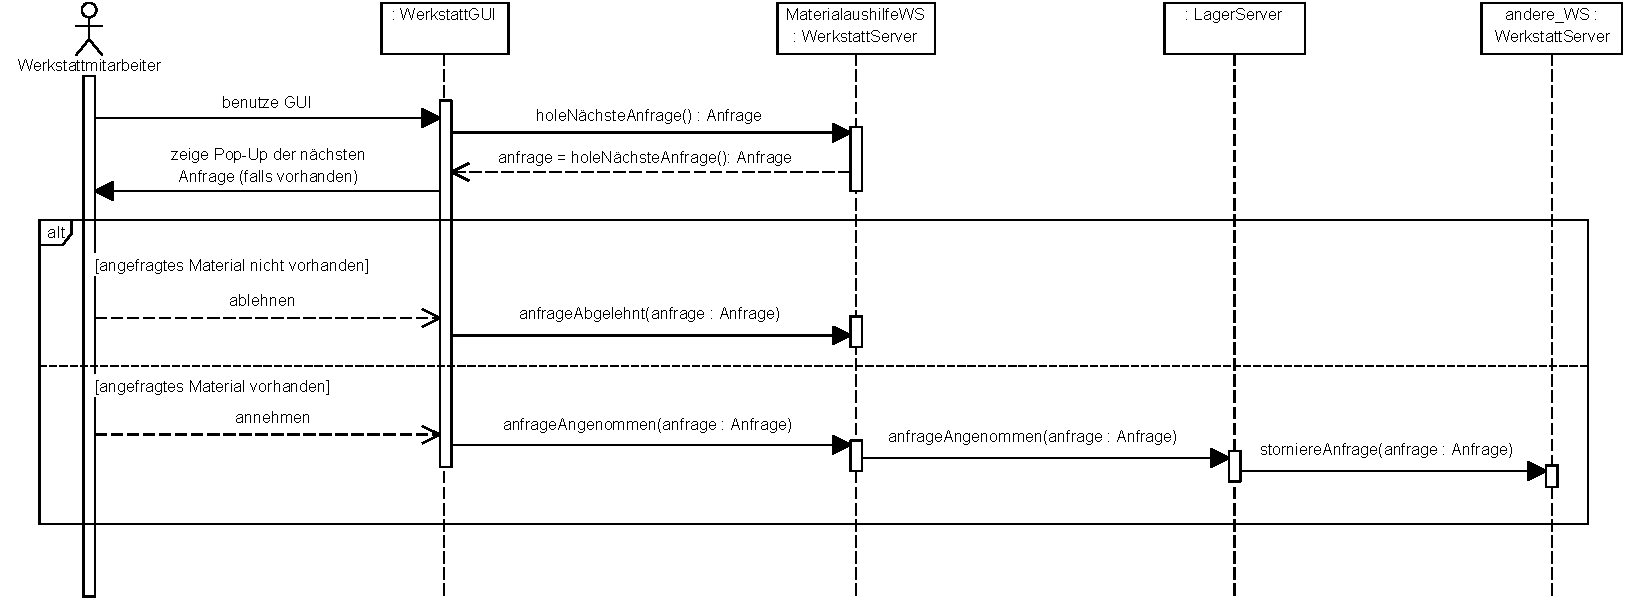
\includegraphics[width=\textwidth]{PDF/Use_Case_3-Materialanfrage_beantworten.pdf}
	\end{frame}
	\begin{frame}{Use Case 4 - Projektvorlage bearbeiten}
		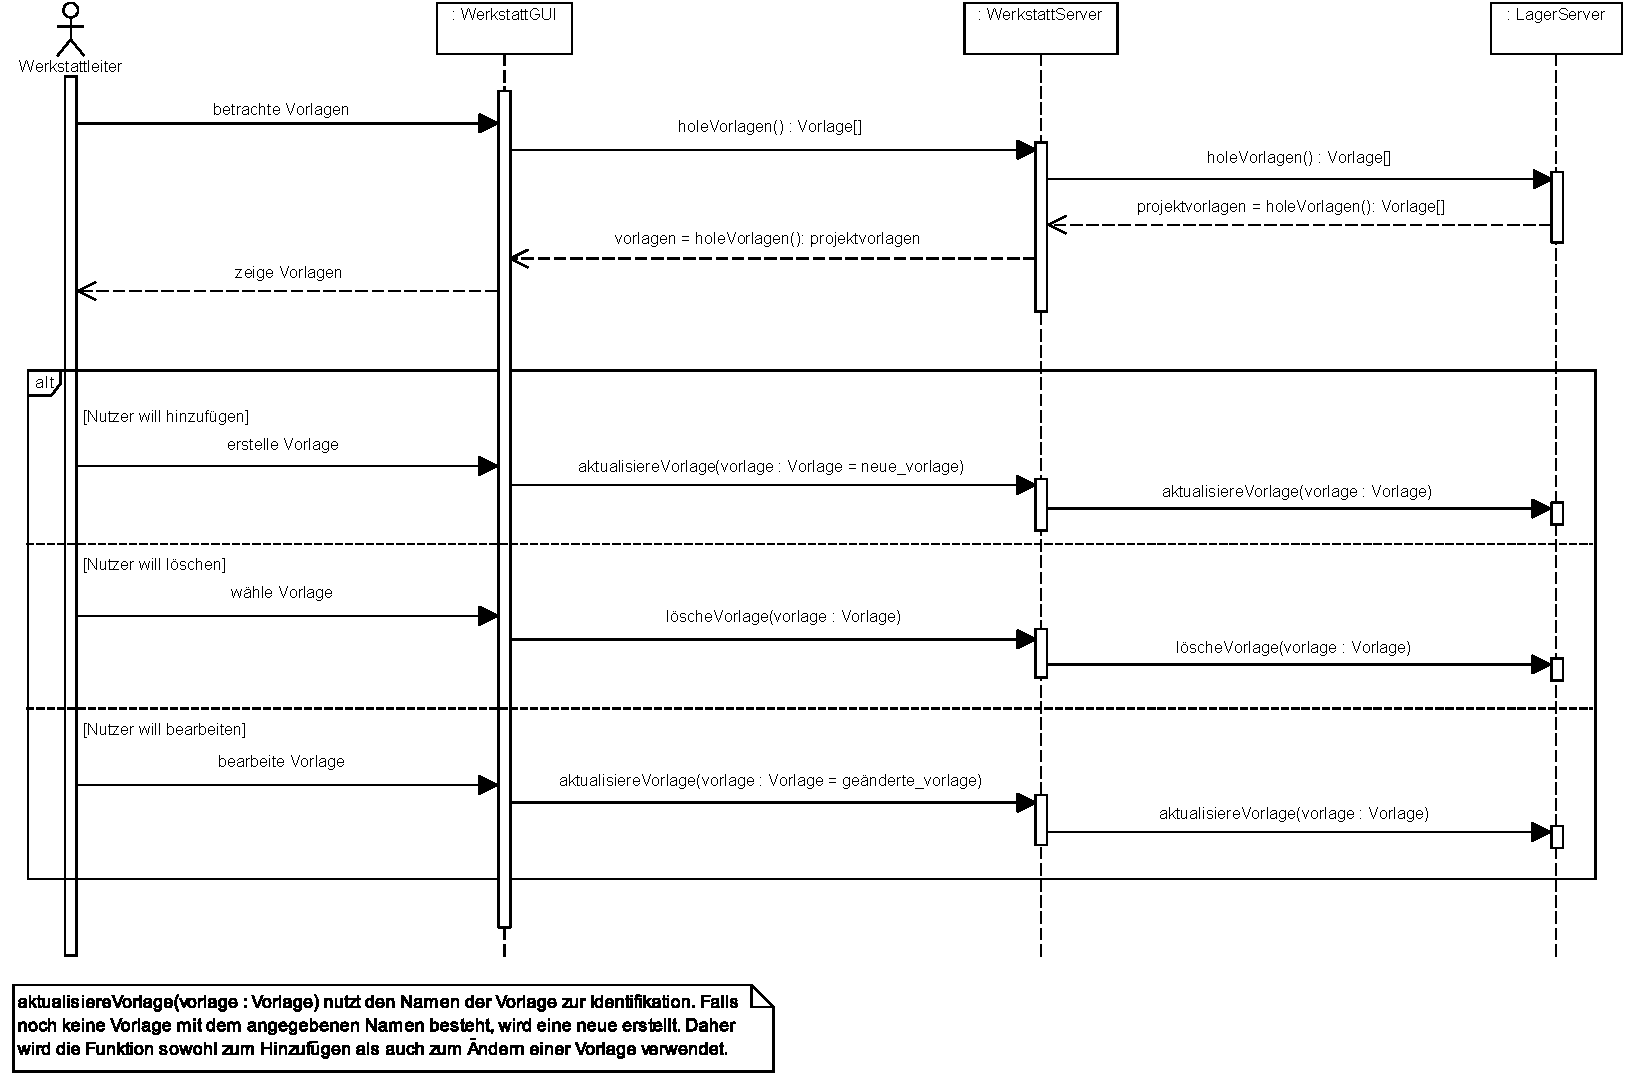
\includegraphics[height=0.75 \textheight]{PDF/Use_Case_4-Projektvorlage_bearbeiten.pdf}
	\end{frame}
		\begin{frame}{Use Case 5 - Sonderbedarf eintragen}
		Ein Werkstattleiter \textbf{trägt Sonderbedarf ein}, welcher aus Materialtyp, Anzahl und Begründung besteht. Der Eintrag wird von der GUI an den Werkstattserver gesendet:\\
\medskip
\texttt{sendeSonderbedarf(material : Materialeintrag, begründung : string)}
\\
\medskip
Der Sonderbedarf wird dort für spätere Verarbeitung gespeichert.
	
	\end{frame}
	\begin{frame}{Use Case 6 - Anforderung abschicken}
		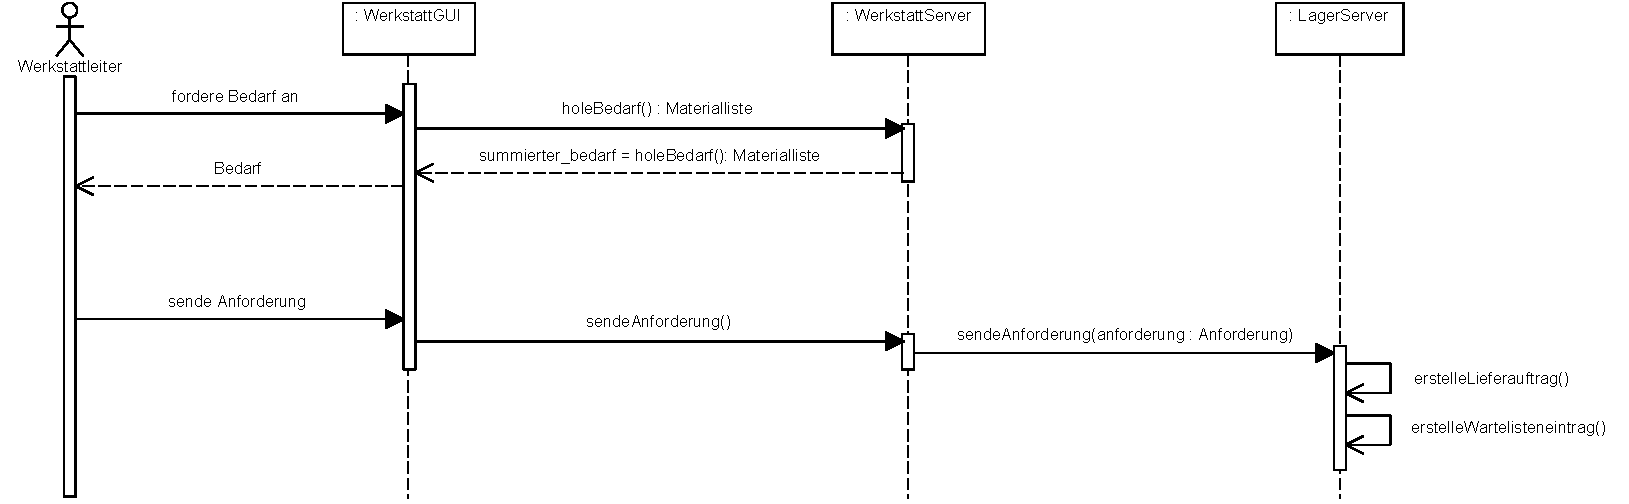
\includegraphics[width=\textwidth]{PDF/Use_Case_6-Anforderung_abschicken.pdf}
	\end{frame}
\begin{frame}{Use Case 7 - Sollbestand festlegen}
Der Werkstattleiter \textbf{ruft die Liste der Vorratsbehältnisse auf} (GUI holt diese von Server):

\texttt{holeBehältnisse() : Vorratsbehältnis[]}

Er wählt ein Vorratsbehältnis aus und \textbf{ändert Sollbestand und/oder Material} oder er \textbf{legt einen neuen Eintrag an}, wobei Kennung, Materialtyp und Sollbestand eingegeben werden müssen.
Für beide Aktionen wird die gleiche Funktion genutzt (GUI übermittelt an Server):

\texttt{aktualisiereBehältnis(behältnis : Vorratsbehältnis)}

Wenn ein Behältnis mit noch nicht existenter Kennung "`aktualisiert"' wird, erstellt der Server einen neuen Eintrag.
\end{frame}
\begin{frame}{Use Case 8 - Anforderung empfangen}
Ein Lagerist nutzt die LagerGUI, welche die \textbf{erfüllbaren Lieferaufträge anfordert} (vom Lagerserver):

\texttt{holeLieferaufträge() : Lieferauftrag []}

Der Server übernimmt dabei die Umrechnung von Stückzahl in Verpackungseinheiten.
Der Lagerist kann eine Anforderung auswählen (nach Wunsch auch ausdrucken) und \textbf{bestätigen}.

\texttt{bestätigeLieferauftrag(auftrag : Lieferauftrag)}

Der Server löscht daraufhin den Lieferauftrag und reduziert den Materialbestand.
\end{frame}
\begin{frame}{Use Case 9 - Wareneingang dokumentieren}
Ein Lagerist betrachtet alle Bestellungen. (GUI holt Bestellungsliste von Lagerserver):

\texttt{holeOffeneBestellungen() : GESBestellbestätigung []}

Er wählt eine Bestellung aus und kann über die GUI dann Vermerke bezüglich gelieferter Anzahl und Zustand eingeben. Dann werden diese \textbf{Vermerke übermittelt} (von der GUI an den Server)

\texttt{dokumentiereWareneingang(bestellung : GESBestellbestätigung, wareneingang : Lieferposition[])}

Der Server ermittelt daraus den neuen Warenbestand und konvertiert ausstehende Anforderungen von der Warteliste in Lieferaufträge, die dann in Use Case 8 abgearbeitet werden können
\end{frame}
\begin{frame}{Use Case 10 - Großhändler bearbeiten}
Ein Lagerist betrachtet über die GUI eine Liste der Großhändler (GUI \textbf{holt Großohändlerliste} von Lagerserver).\\
\medskip
\texttt{holeGroßhändlerliste() : Großhändlerkontakt[]}\\
\medskip
Er kann einen \textbf{Großhändler löschen} oder einen \textbf{Großhändler aktualisieren bzw. neuerstellen}, wobei der Name eines bestehenden Großhändlers nicht geändert werden kann und zum Erstellen eines neuen Großhändlers einfach ein noch nicht vorhandener Name eingegeben wird.
Eine entsprechende Anfrage wird von der GUI an den Lagerserver gesendet:\\
\medskip
\texttt{löscheGroßhändlerkontakt(großhändler : Großhändlerkontakt)} \\
\medskip
\texttt{aktualisiereGroßhändlerkontakt(großhändler : Großhändlerkontakt)}\\
\medskip

Ein Großhändlerkontakt Eintrag beinhaltet Name, Kontakt, Kontodaten, IP-Adresse und die Artikelbezeichnungen.
\end{frame}
\begin{frame}{Use Case 11 - Bedarf identifizieren}
Wenn es Montag früh ist oder eine dringende Bestellung angefordert wurde, \textbf{holt die GUI die Bedarfsliste von Lagerserver} und zeigt sie dem Lagerist:

\texttt{holeBedarf() : Materialliste}

Die Materialliste kann ausgedruckt werden.
\end{frame}
	\begin{frame}{Use Case 12 - Bestellung aufgeben}
		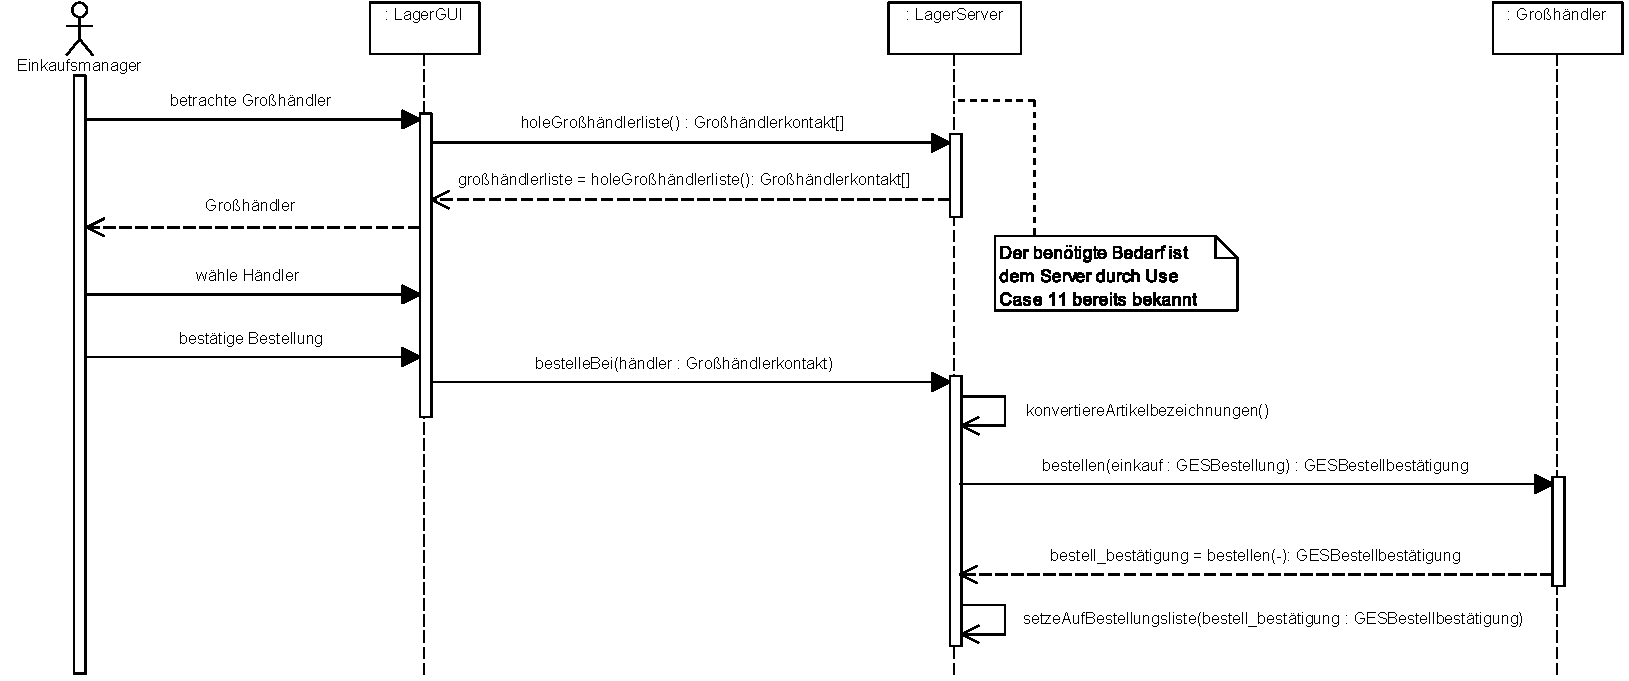
\includegraphics[width=\textwidth]{PDF/Use_Case_12-Bestellung_aufgeben.pdf}
	\end{frame}
\begin{frame}{Use Case 13 - Lagermengen bearbeiten}
Ein Einkaufsmanager kann in der Lager-GUI eine \textbf{Liste aller gelagerten Materialien aufrufen} (beinhaltet jeweiligen Sollbestand):

\texttt{holeVorratsliste() : Materialvorrat []}

Für alle Materialien kann er einen \textbf{Sollbestand festlegen}, der dann an den Server übertragen wird. Es wird dabei der gesamte Materialeintrag übertragen, wobei der Server das geänderte Material anhand des Typs identifiziert. Dass nur der Sollbestand, nicht aber z.B. die Packungsgröße geändert werden kann, ist Aufgabe der GUI:

\texttt{aktualisiereMaterialvorrat(geänderter\_Materialvorrat : Materialvorrat)}
\end{frame}
	\section{Komponentenschnittstellen}
	\begin{frame}{Komponentenschnittstellen}
		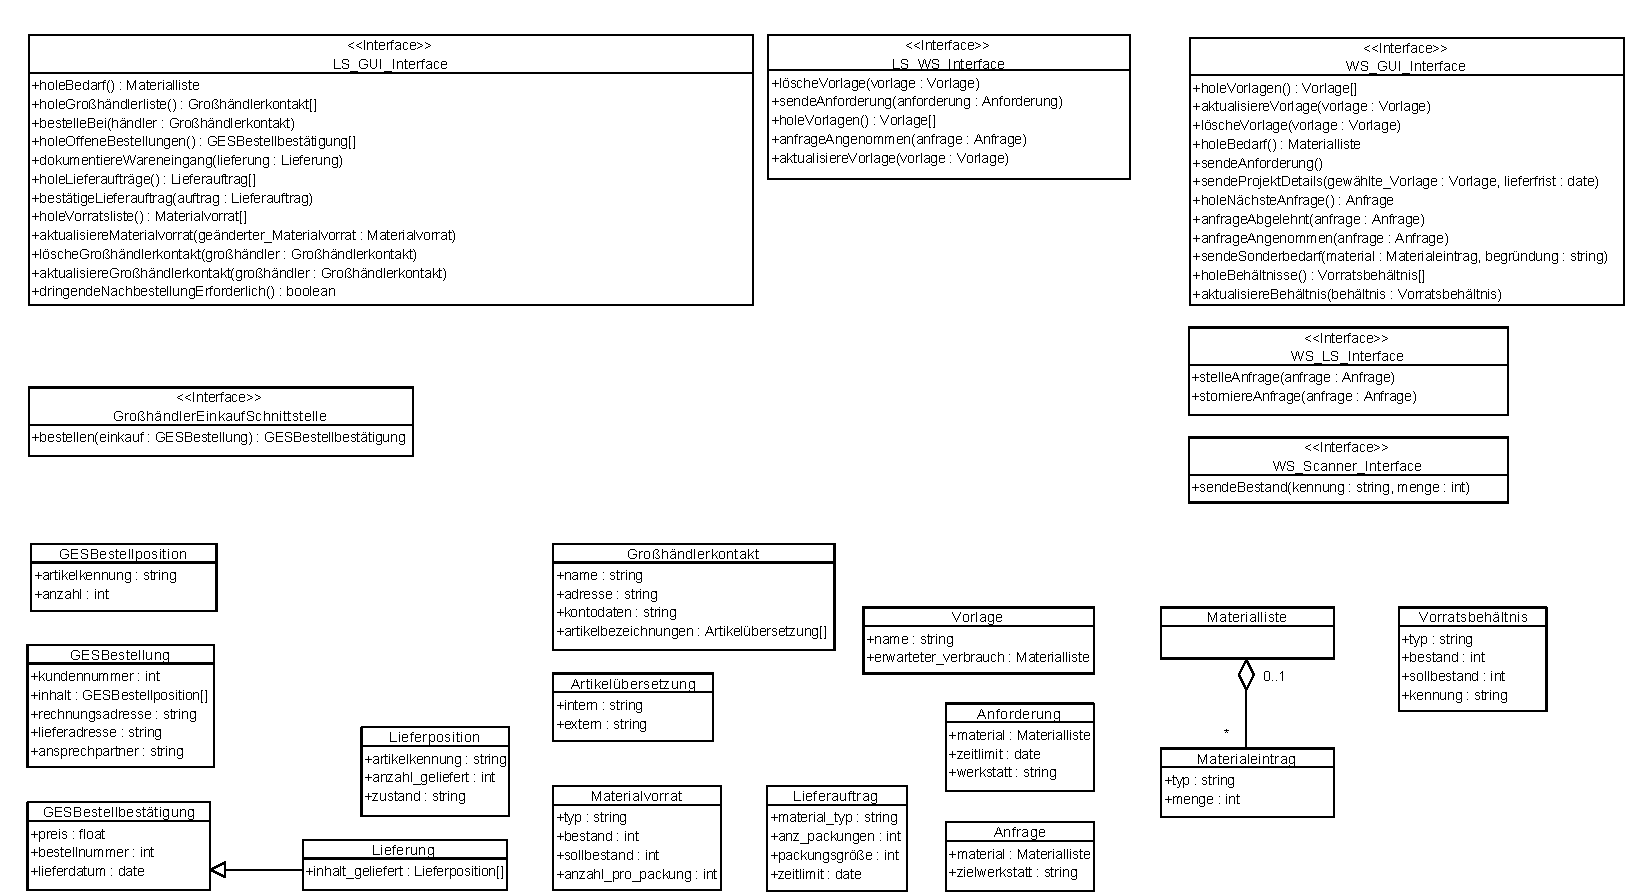
\includegraphics[width=\textwidth]{PDF/Schnittstellen.pdf}
	\end{frame}
	\section{Konkrete Architektur}
	\begin{frame}{Konkrete Architektur}
		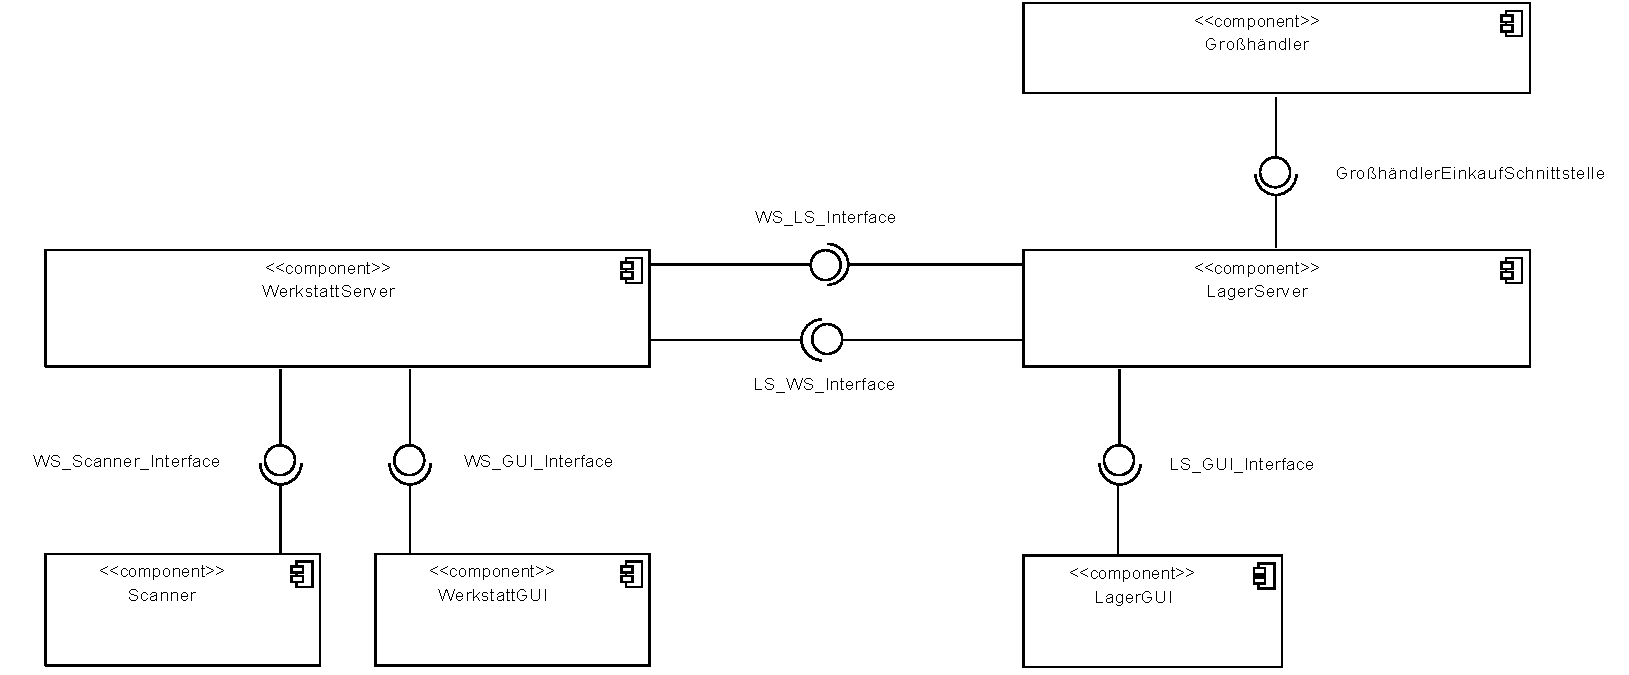
\includegraphics[width=\textwidth]{PDF/Konkrete_Architektur.pdf}
	\end{frame}
	\section{ Innere Struktur der Komponenten}
	\begin{frame}{Innere Struktur des Werkstattservers}
		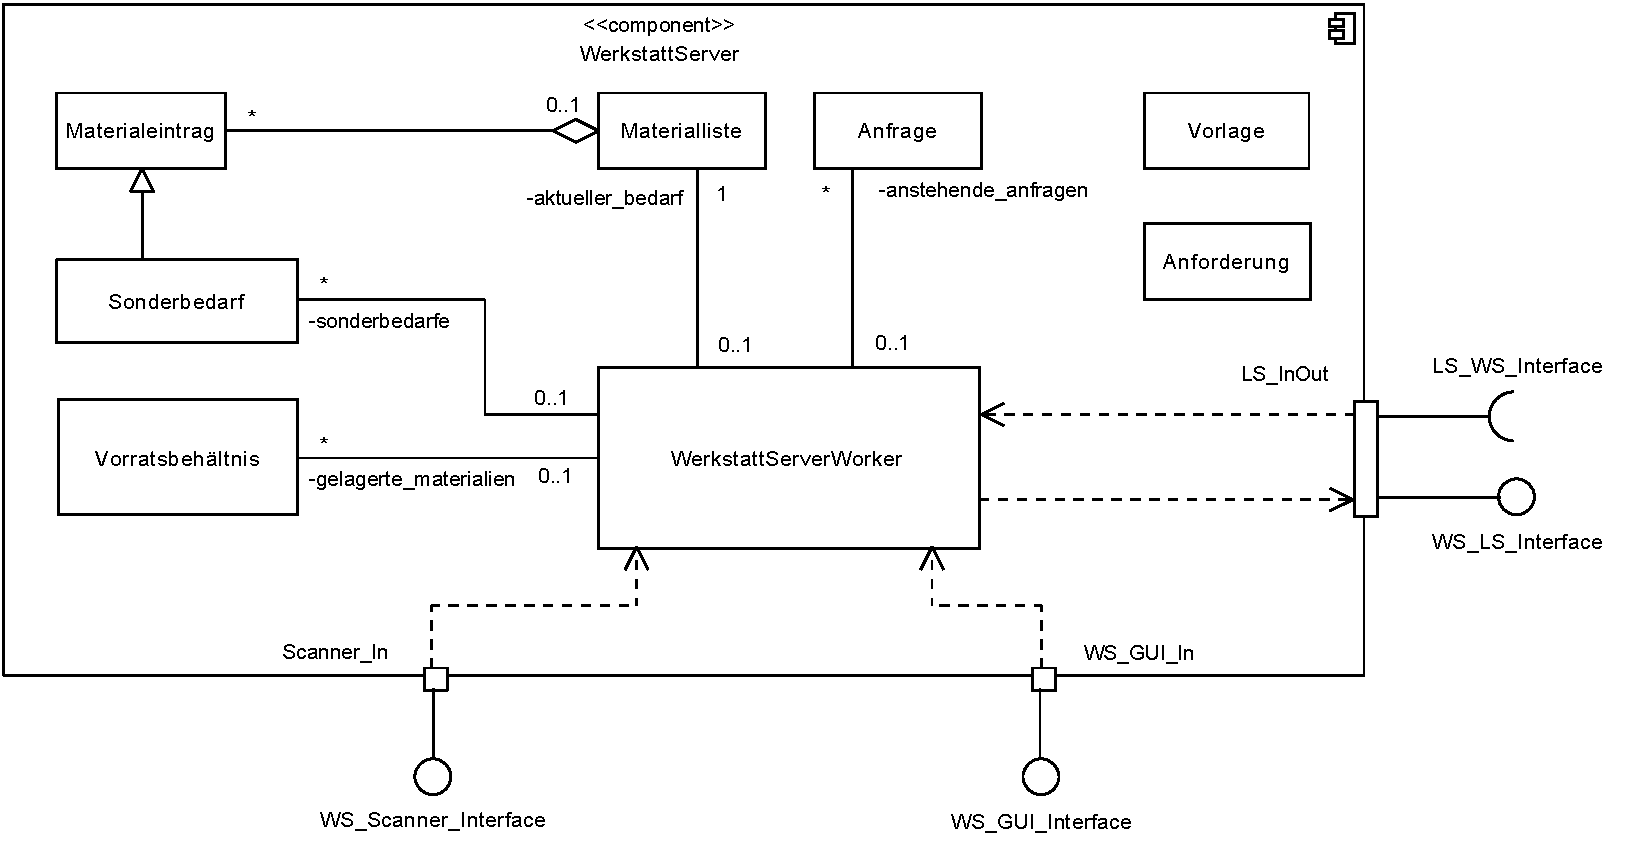
\includegraphics[width=\textwidth]{PDF/WS_Innere_Struktur.pdf}
	\end{frame}
	\begin{frame}{Innere Struktur des Werkstattservers}
		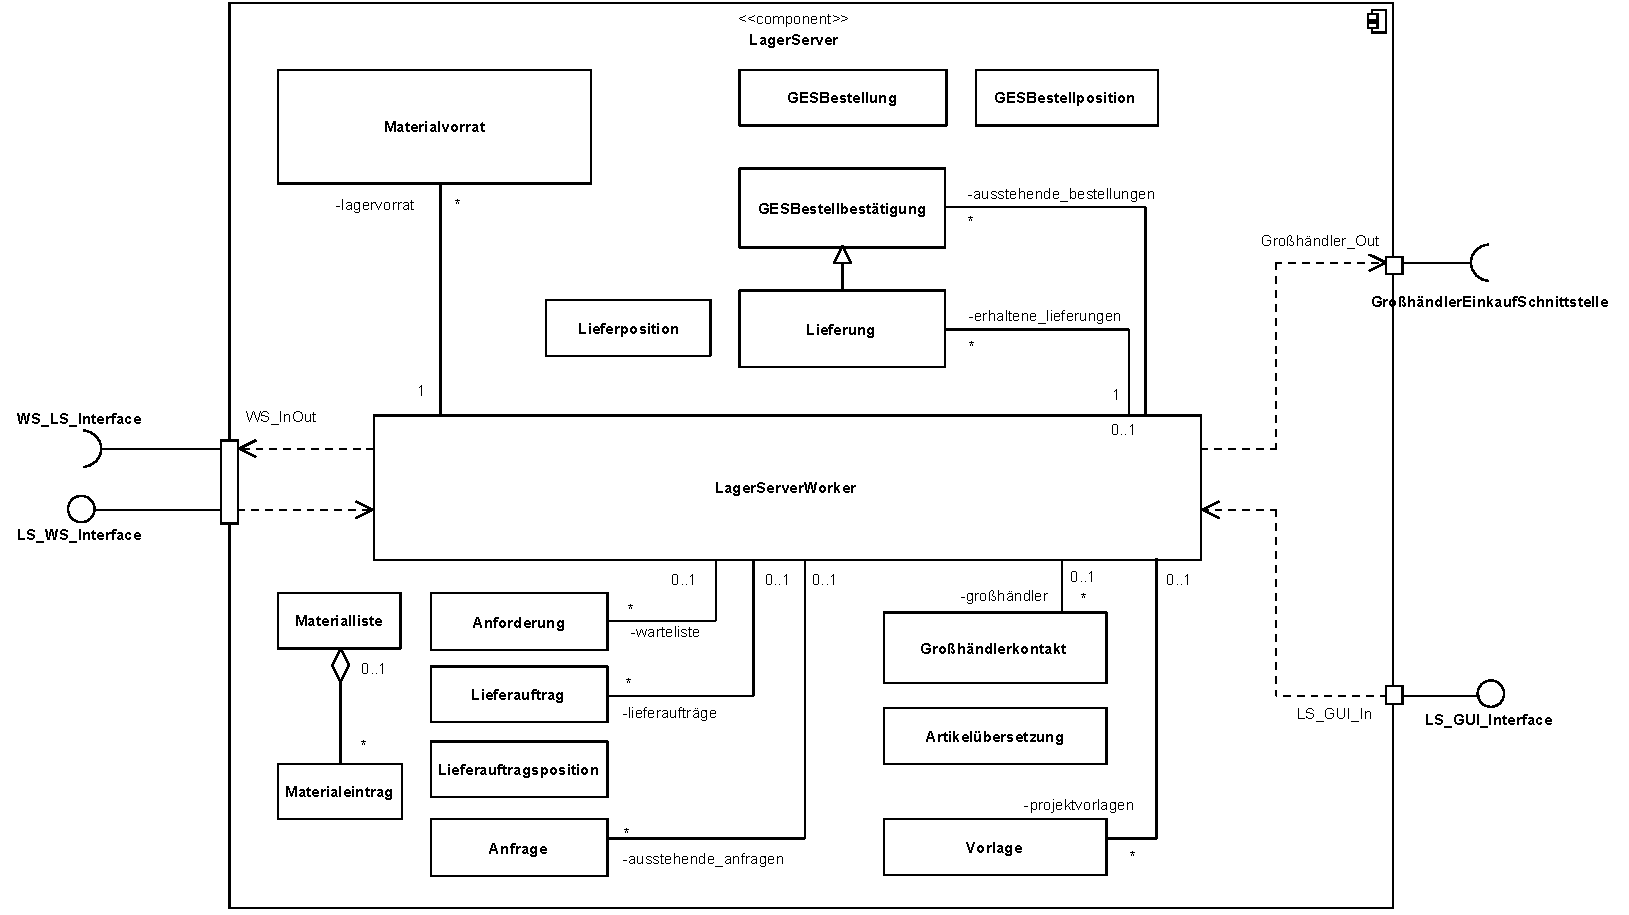
\includegraphics[width=\textwidth]{PDF/LS_Innere_Struktur.pdf}
	\end{frame}
	\section{Paketstruktur}
	\begin{frame}{Paketstruktur}
		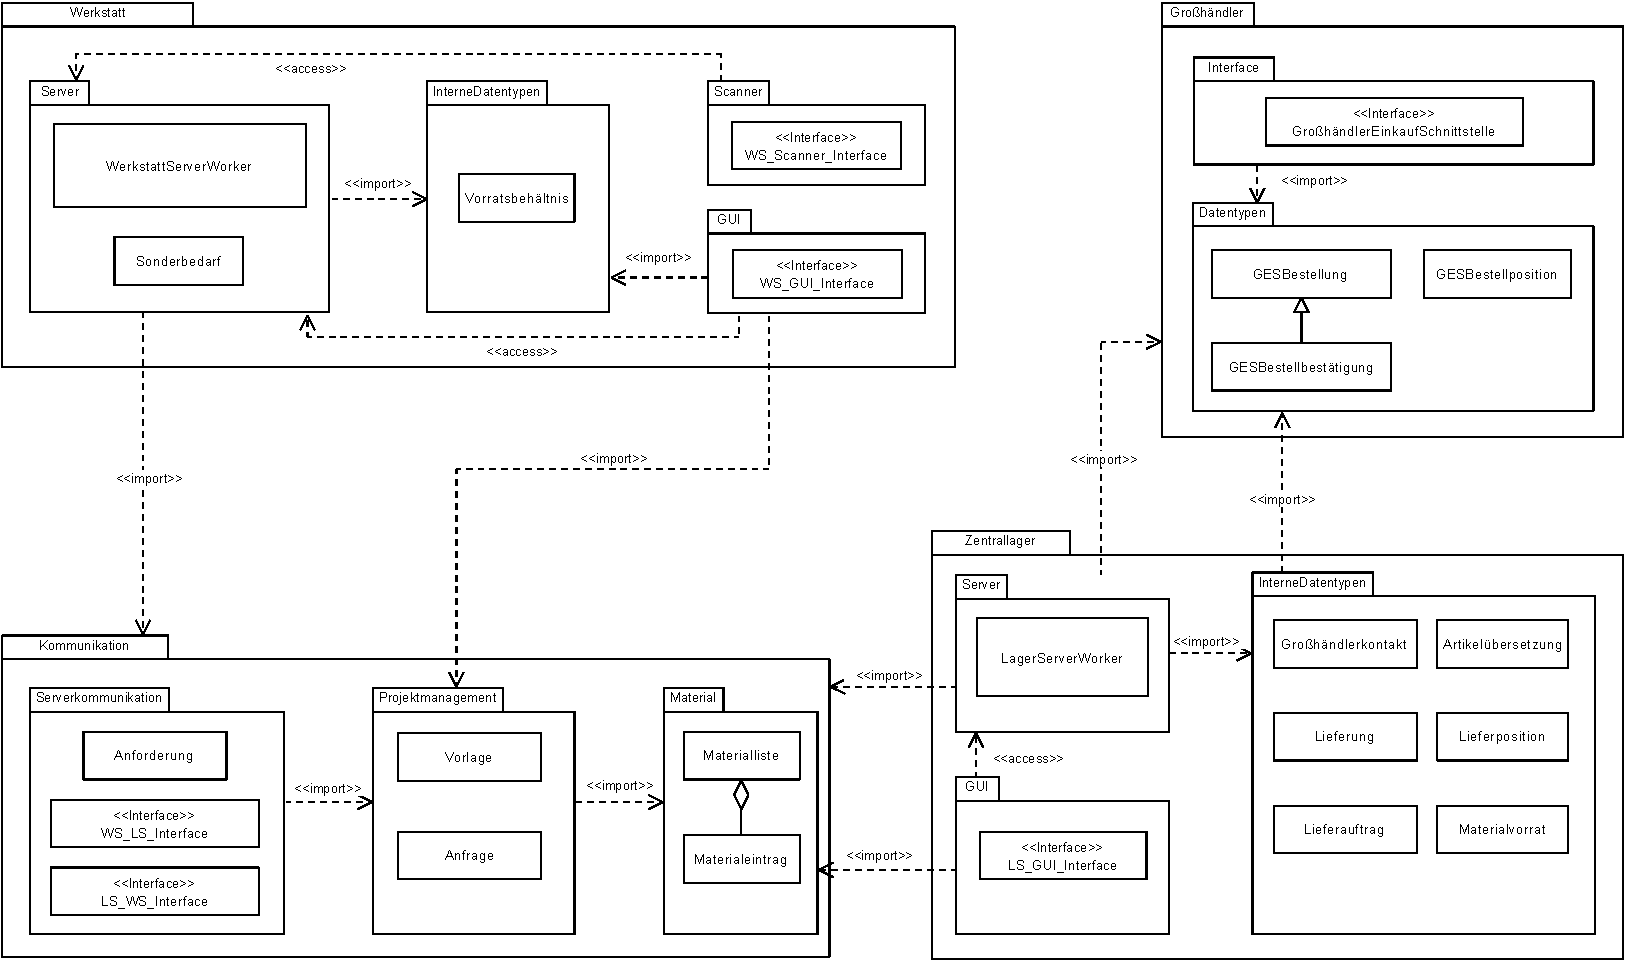
\includegraphics[height=0.75 \textheight]{PDF/Paket_Struktur.pdf}
	\end{frame}
	\section{Paketdetails}
	\begin{frame}{Paketdetails}
		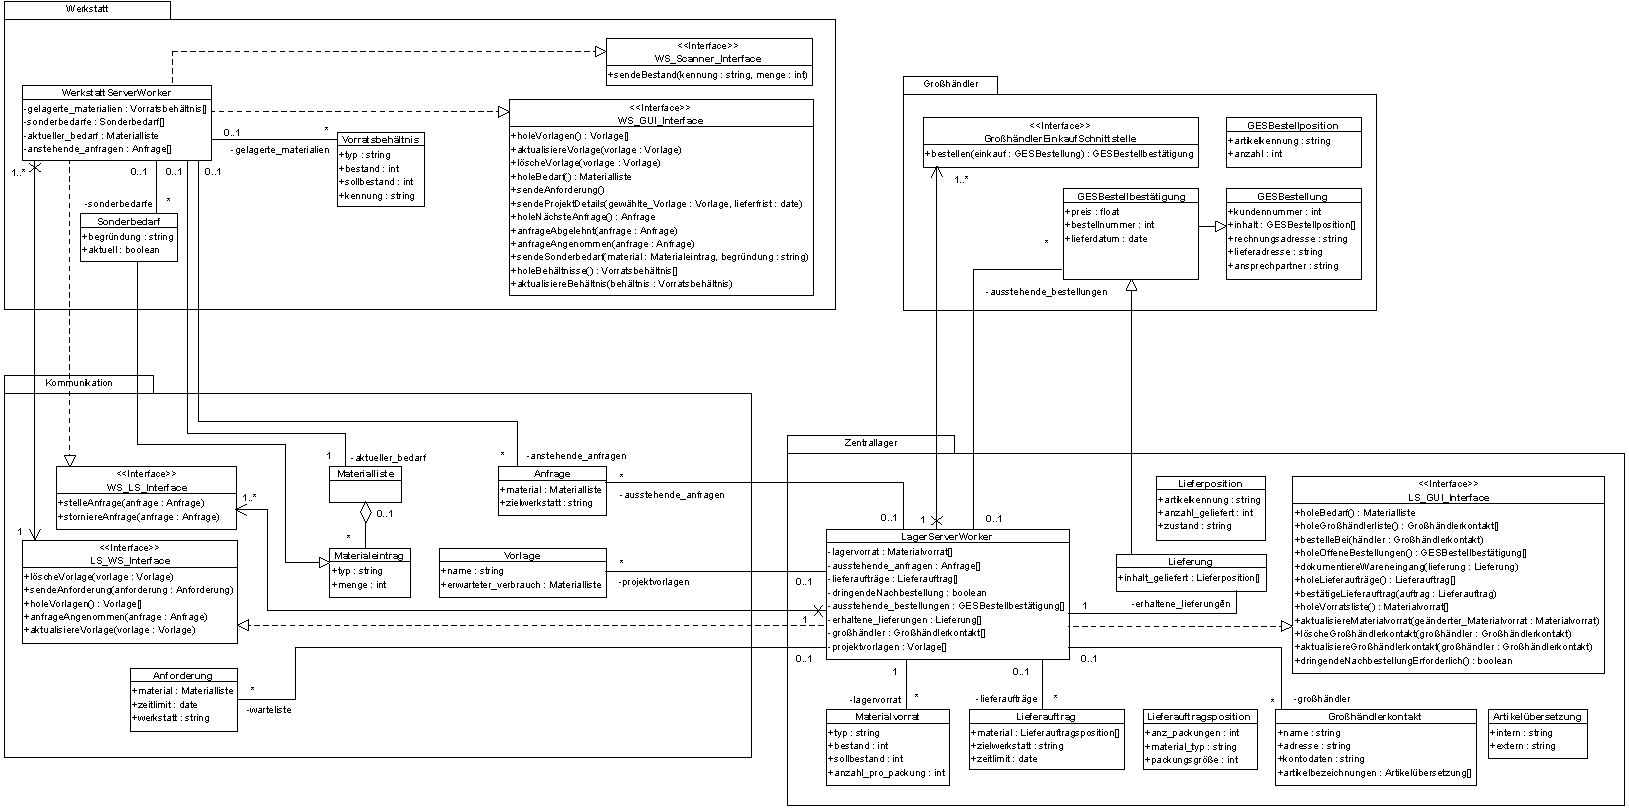
\includegraphics[width=\textwidth]{PDF/Paketdetails.pdf}
	\end{frame}
\begin{frame}{Detailansicht - Werkstatt}
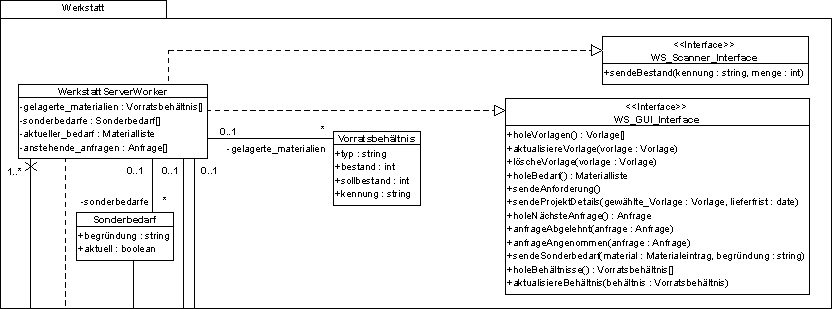
\includegraphics[width=\textwidth]{PDF/Werkstatt_Paket.pdf}
\end{frame}
\begin{frame}{Detailansicht - Kommunikation}
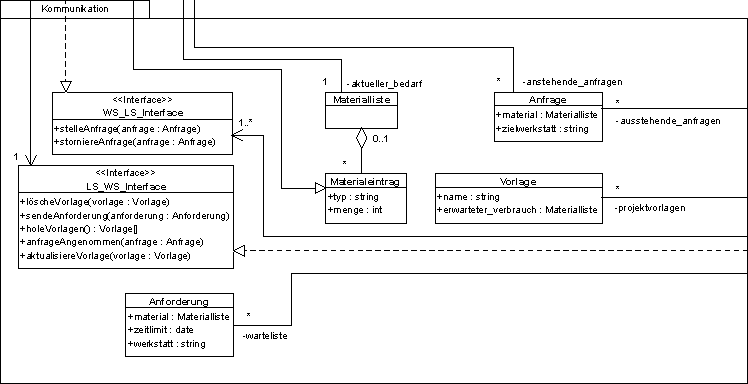
\includegraphics[width=\textwidth]{PDF/Kommunikation_Paket.pdf}
\end{frame}
\begin{frame}{Detailansicht - Zentrallager}
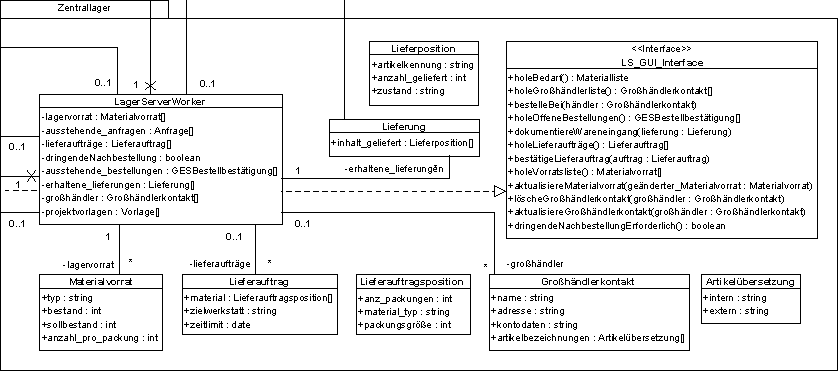
\includegraphics[width=\textwidth]{PDF/Zentrallager_Paket.pdf}
\end{frame}
\begin{frame}{Detailansicht - Großhändler}
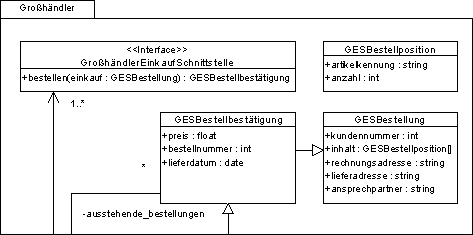
\includegraphics[width=\textwidth]{PDF/GH_Paket.pdf}
\end{frame}
	\begin{frame}[title=Hauptgebaeude_Nacht.jpg]
		\maketitle
		\date{26. Mai 2018}
	\end{frame}
\end{document}

